%% abtex2-modelo-trabalho-academico.tex, v-1.9.7 laurocesar
%% Copyright 2012-2018 by abnTeX2 group at http://www.abntex.net.br/ 
%%
%% This work may be distributed and/or modified under the
%% conditions of the LaTeX Project Public License, either version 1.3
%% of this license or (at your option) any later version.
%% The latest version of this license is in
%%   http://www.latex-project.org/lppl.txt
%% and version 1.3 or later is part of all distributions of LaTeX
%% version 2005/12/01 or later.
%%
%% This work has the LPPL maintenance status `maintained'.
%% 
%% The Current Maintainer of this work is the abnTeX2 team, led
%% by Lauro César Araujo. Further information are available on 
%% http://www.abntex.net.br/
%%
%% This work consists of the files abntex2-modelo-trabalho-academico.tex,
%% abntex2-modelo-include-comandos and abntex2-modelo-references.bib
%%

% ------------------------------------------------------------------------
% ------------------------------------------------------------------------
% abnTeX2: Modelo de Trabalho Academico (tese de doutorado, dissertacao de
% mestrado e trabalhos monograficos em geral) em conformidade com 
% ABNT NBR 14724:2011: Informacao e documentacao - Trabalhos academicos -
% Apresentacao
% ------------------------------------------------------------------------
% ------------------------------------------------------------------------

\documentclass[
	% -- opções da classe memoir --
	12pt,				% tamanho da fonte
	openright,			% capítulos começam em pág ímpar (insere página vazia caso preciso)
	twoside,			% para impressão em recto e verso. Oposto a oneside
	a4paper,			% tamanho do papel. 
	% -- opções da classe abntex2 --
	%chapter=TITLE,		% títulos de capítulos convertidos em letras maiúsculas
	%section=TITLE,		% títulos de seções convertidos em letras maiúsculas
	%subsection=TITLE,	% títulos de subseções convertidos em letras maiúsculas
	%subsubsection=TITLE,% títulos de subsubseções convertidos em letras maiúsculas
	% -- opções do pacote babel --
	english,			% idioma adicional para hifenização
	french,				% idioma adicional para hifenização
	spanish,			% idioma adicional para hifenização
	brazil				% o último idioma é o principal do documento
	]{abntex2}

% ---
% Pacotes básicos 
% ---
\usepackage{lmodern}			% Usa a fonte Latin Modern			
\usepackage[T1]{fontenc}		% Selecao de codigos de fonte.
\usepackage[utf8]{inputenc}		% Codificacao do documento (conversão automática dos acentos)
\usepackage{indentfirst}		% Indenta o primeiro parágrafo de cada seção.
\usepackage{color}				% Controle das cores
\usepackage{graphicx}			% Inclusão de gráficos
\usepackage{microtype} 			% para melhorias de justificação
% ---
		
% ---
% Pacotes adicionais, usados apenas no âmbito do Modelo Canônico do abnteX2
% ---
\usepackage{lipsum}				% para geração de dummy text
% ---

% ---
% Pacotes de citações
% ---
\usepackage[brazilian,hyperpageref]{backref}	 % Paginas com as citações na bibl
\usepackage[alf]{abntex2cite}	% Citações padrão ABNT

% --- 
% CONFIGURAÇÕES DE PACOTES
% --- 
\graphicspath{ {images/} } %definindo localização das imagens
% ---
% Configurações do pacote backref
% Usado sem a opção hyperpageref de backref
\renewcommand{\backrefpagesname}{Citado na(s) página(s):~}
% Texto padrão antes do número das páginas
\renewcommand{\backref}{}
% Define os textos da citação
\renewcommand*{\backrefalt}[4]{
	\ifcase #1 %
		Nenhuma citação no texto.%
	\or
		Citado na página #2.%
	\else
		Citado #1 vezes nas páginas #2.%
	\fi}%
% ---

% ---
% Informações de dados para CAPA e FOLHA DE ROSTO
% ---
\titulo{Sistema de Recomendação para Técnicas de Tolerância a Falhas em Ambientes de Nuvem}
\autor{Pedrenrique Gonçalves Guimarães}
\local{São José do Rio Preto, SP}
\data{2019}
\orientador{Aleardo Manacero Junior}
\instituicao{%
  Universidade Estadual Paulista ``Júlio de Mesquita Filho'' - UNESP
  \par
  Instituto de Biociências, Letras e Ciências Exatas - IBILCE
  \par
  Departamento de Ciências de Computação e Estatística}
\tipotrabalho{Tese (Graduação)}
% O preambulo deve conter o tipo do trabalho, o objetivo, 
% o nome da instituição e a área de concentração 
\preambulo{Modelo canônico de trabalho monográfico acadêmico em conformidade com
as normas ABNT apresentado à comunidade de usuários \LaTeX.}
% ---


% ---
% Configurações de aparência do PDF final

% alterando o aspecto da cor azul
\definecolor{blue}{RGB}{41,5,195}

% informações do PDF
\makeatletter
\hypersetup{
     	%pagebackref=true,
		pdftitle={\@title}, 
		pdfauthor={\@author},
    	pdfsubject={\imprimirpreambulo},
	    pdfcreator={LaTeX with abnTeX2},
		pdfkeywords={abnt}{latex}{abntex}{abntex2}{trabalho acadêmico}, 
		colorlinks=true,       		% false: boxed links; true: colored links
    	linkcolor=blue,          	% color of internal links
    	citecolor=blue,        		% color of links to bibliography
    	filecolor=magenta,      		% color of file links
		urlcolor=blue,
		bookmarksdepth=4
}
\makeatother
% --- 

% ---
% Posiciona figuras e tabelas no topo da página quando adicionadas sozinhas
% em um página em branco. Ver https://github.com/abntex/abntex2/issues/170
\makeatletter
\setlength{\@fptop}{5pt} % Set distance from top of page to first float
\makeatother
% ---

% ---
% Possibilita criação de Quadros e Lista de quadros.
% Ver https://github.com/abntex/abntex2/issues/176
%
\newcommand{\quadroname}{Quadro}
\newcommand{\listofquadrosname}{Lista de quadros}

\newfloat[chapter]{quadro}{loq}{\quadroname}
\newlistof{listofquadros}{loq}{\listofquadrosname}
\newlistentry{quadro}{loq}{0}

% configurações para atender às regras da ABNT
\setfloatadjustment{quadro}{\centering}
\counterwithout{quadro}{chapter}
\renewcommand{\cftquadroname}{\quadroname\space} 
\renewcommand*{\cftquadroaftersnum}{\hfill--\hfill}

\setfloatlocations{quadro}{hbtp} % Ver https://github.com/abntex/abntex2/issues/176
% ---

% --- 
% Espaçamentos entre linhas e parágrafos 
% --- 

% O tamanho do parágrafo é dado por:
\setlength{\parindent}{1.3cm}

% Controle do espaçamento entre um parágrafo e outro:
\setlength{\parskip}{0.2cm}  % tente também \onelineskip

% ---
% compila o indice
% ---
\makeindex
% ---

% ----
% Início do documento
% ----
\begin{document}

% Seleciona o idioma do documento (conforme pacotes do babel)
%\selectlanguage{english}
\selectlanguage{brazil}

% Retira espaço extra obsoleto entre as frases.
\frenchspacing 

% ----------------------------------------------------------
% ELEMENTOS PRÉ-TEXTUAIS
% ----------------------------------------------------------
% \pretextual

% ---
% Capa
% ---
\imprimircapa
% ---

% ---
% Folha de rosto
% (o * indica que haverá a ficha bibliográfica)
% ---
\imprimirfolhaderosto*
% ---

% ---
% Inserir a ficha bibliografica
% ---

% Isto é um exemplo de Ficha Catalográfica, ou ``Dados internacionais de
% catalogação-na-publicação''. Você pode utilizar este modelo como referência. 
% Porém, provavelmente a biblioteca da sua universidade lhe fornecerá um PDF
% com a ficha catalográfica definitiva após a defesa do trabalho. Quando estiver
% com o documento, salve-o como PDF no diretório do seu projeto e substitua todo
% o conteúdo de implementação deste arquivo pelo comando abaixo:
%
% \begin{fichacatalografica}
%     \includepdf{fig_ficha_catalografica.pdf}
% \end{fichacatalografica}

\begin{fichacatalografica}
	\sffamily
	\vspace*{\fill}					% Posição vertical
	\begin{center}					% Minipage Centralizado
	\fbox{\begin{minipage}[c][8cm]{13.5cm}		% Largura
	\small
	\imprimirautor
	%Sobrenome, Nome do autor
	
	\hspace{0.5cm} \imprimirtitulo  / \imprimirautor. --
	\imprimirlocal, \imprimirdata-
	
	\hspace{0.5cm} \thelastpage p. : il. (algumas color.) ; 30 cm.\\
	
	\hspace{0.5cm} \imprimirorientadorRotulo~\imprimirorientador\\
	
	\hspace{0.5cm}
	\parbox[t]{\textwidth}{\imprimirtipotrabalho~--~\imprimirinstituicao,
	\imprimirdata.}\\
	
	\hspace{0.5cm}
		1. Palavra-chave1.
		2. Palavra-chave2.
		2. Palavra-chave3.
		I. Orientador.
		II. Universidade xxx.
		III. Faculdade de xxx.
		IV. Título 			
	\end{minipage}}
	\end{center}
\end{fichacatalografica}
% ---

% ---
% Inserir errata
% ---
%\begin{errata}
%Elemento opcional da \citeonline[4.2.1.2]{NBR14724:2011}. Exemplo:
%
%\vspace{\onelineskip}

%FERRIGNO, C. R. A. \textbf{Tratamento de neoplasias ósseas apendiculares com
%reimplantação de enxerto ósseo autólogo autoclavado associado ao plasma
%rico em plaquetas}: estudo crítico na cirurgia de preservação de membro em
%cães. 2011. 128 f. Tese (Livre-Docência) - Faculdade de Medicina Veterinária e
%Zootecnia, Universidade de São Paulo, São Paulo, 2011.

%\begin{table}[htb]
%\center
%\footnotesize
%\begin{tabular}{|p{1.4cm}|p{1cm}|p{3cm}|p{3cm}|}
%  \hline
%   \textbf{Folha} & \textbf{Linha}  & \textbf{Onde se lê}  & \textbf{Leia-se}  \\
%    \hline
%    1 & 10 & auto-conclavo & autoconclavo\\
%   \hline
%\end{tabular}
%\end{table}
%
%\end{errata}
% ---

% ---
% Inserir folha de aprovação
% ---

% Isto é um exemplo de Folha de aprovação, elemento obrigatório da NBR
% 14724/2011 (seção 4.2.1.3). Você pode utilizar este modelo até a aprovação
% do trabalho. Após isso, substitua todo o conteúdo deste arquivo por uma
% imagem da página assinada pela banca com o comando abaixo:
%
% \begin{folhadeaprovacao}
% \includepdf{folhadeaprovacao_final.pdf}
% \end{folhadeaprovacao}
%
\begin{folhadeaprovacao}

  \begin{center}
    {\ABNTEXchapterfont\large\imprimirautor}

    \vspace*{\fill}\vspace*{\fill}
    \begin{center}
      \ABNTEXchapterfont\bfseries\Large\imprimirtitulo
    \end{center}
    \vspace*{\fill}
    
    \hspace{.45\textwidth}
    \begin{minipage}{.5\textwidth}
        \imprimirpreambulo
    \end{minipage}%
    \vspace*{\fill}
   \end{center}
        
   Trabalho aprovado. \imprimirlocal, %24 de novembro de 2012:

   \assinatura{\textbf{\imprimirorientador} \\ Orientador} 
   \assinatura{\textbf{Renata Spolon Lobato} \\ Convidado 1}
   \assinatura{\textbf{Rodrigo Capobianco Guido} \\ Convidado 2}
   %\assinatura{\textbf{Professor} \\ Convidado 3}
   %\assinatura{\textbf{Professor} \\ Convidado 4}
      
   \begin{center}
    \vspace*{0.5cm}
    {\large\imprimirlocal}
    \par
    {\large\imprimirdata}
    \vspace*{1cm}
  \end{center}
  
\end{folhadeaprovacao}
% ---

% ---
% Dedicatória
% ---
\begin{dedicatoria}
   \vspace*{\fill}
   \centering
   \noindent
   \textit{ Inserir dedicatória aqui} \vspace*{\fill}
\end{dedicatoria}
% ---

% ---
% Agradecimentos
% ---
\begin{agradecimentos}


\end{agradecimentos}
% ---

% ---
% Epígrafe
% ---
\begin{epigrafe}
    \vspace*{\fill}
	\begin{flushright}
		\textit{Epígrafo}
	\end{flushright}
\end{epigrafe}
% ---

% ---
% RESUMOS
% ---

% resumo em português
\setlength{\absparsep}{18pt} % ajusta o espaçamento dos parágrafos do resumo
\begin{resumo}
 A computação em nuvem tem ganhado grande popularidade nos últimos anos por oferecer uma gama de serviços e recursos diversificados de forma rápida, prática e bastante acessível para o público casual e também empresarial. Tais sistemas têm como principais características a escalabilidade e alta carga de trabalho, na maioria dos casos. Entretanto, as plataformas em nuvem também estão bastante suscetíveis a diversos tipos de falhas que podem comprometer o funcionamento dos serviços, de sua infraestrutura e de todo o sistema que os comporta, permitindo assim uma perda de dados massiva e possível interrupção de suas atividades por tempo indeterminado. Tais ambientes devem possuir uma boa tolerância a essas falhas, o que significa dizer que a equipe por trás desse ambiente deve ser capaz de identificar e resolver quaisquer falhas de forma a não deixar que estas comprometam o ambiente em questão. Para tratamento de tais falhas, existem diversas técnicas que buscam tratar tais problemas, incluindo uma sistematização em classes com as falhas mais comuns.
 Este trabalho visa expandir tal sistematização, utilizando um sistema de recomendação inteligente para que o sistema consiga fazer a sugestão das técnicas corretas para o tratamento de falhas no ambiente de forma automática.

 \textbf{Palavras-chave}: Computação em nuvem, tolerância a falhas, inteligência artificial, sistema de recomendação.
\end{resumo}

% resumo em inglês
\begin{resumo}[Abstract]
 \begin{otherlanguage*}{english}
   This is the english abstract.

   \vspace{\onelineskip}
 
   \noindent 
   \textbf{Keywords}: latex. abntex. text editoration.
 \end{otherlanguage*}
\end{resumo}

% ---
% inserir lista de ilustrações
% ---
\pdfbookmark[0]{\listfigurename}{lof}
\listoffigures*
\cleardoublepage
% ---

% ---
% inserir lista de quadros
% ---
\pdfbookmark[0]{\listofquadrosname}{loq}
\listofquadros*
\cleardoublepage
% ---

% ---
% inserir lista de tabelas
% ---
\pdfbookmark[0]{\listtablename}{lot}
\listoftables*
\cleardoublepage
% ---

% ---
% inserir lista de abreviaturas e siglas
% ---
\begin{siglas}
  \item[ABNT] Associação Brasileira de Normas Técnicas
  \item[abnTeX] ABsurdas Normas para TeX
\end{siglas}
% ---

% ---
% inserir lista de símbolos
% ---
\begin{simbolos}
  \item[$ \Gamma $] Letra grega Gama
  \item[$ \Lambda $] Lambda
  \item[$ \zeta $] Letra grega minúscula zeta
  \item[$ \in $] Pertence
\end{simbolos}
% ---

% ---
% inserir o sumario
% ---
\pdfbookmark[0]{\contentsname}{toc}
\tableofcontents*
\cleardoublepage
% ---



% ----------------------------------------------------------
% ELEMENTOS TEXTUAIS
% ----------------------------------------------------------
\textual

% ----------------------------------------------------------
% Introdução (exemplo de capítulo sem numeração, mas presente no Sumário)
% ----------------------------------------------------------
\chapter{Introdução}
% ----------------------------------------------------------
A computação em nuvem é uma forma de computação que provê diversos serviços distintos por meio da Internet, de forma que o usuário em questão possa acessar os serviços de qualquer plataforma, desde que possua uma conexão com a Internet. Esse tipo de computação tem se tornado muito popular com a expansão da rede mundial de computadores pelo mundo, e com o pesado investimento em infraestutura proporcionado pelas grandes corporações e operadoras de telecomunicações, que agora tornaram mais acessível ao usuário final o acesso a uma conexão rápida e estável, o que é um requisito fundamental para o correto funcionamento desses serviços.

Gigantes da computação como a Amazon, Google, IBM e Microsoft têm investido pesado em infraestrutura para oferecimento de serviços de computação em nuvem \cite{tsai2010service}\cite{lohr2007google}. Outras empresas ganharam grande notoriedade na indústria por oferecerem exclusivamente serviços de computação em nuvem, como é o caso da Netflix, Hulu e Dropbox, por exemplo \cite{berman2012cloud}. 

A alta demanda por tais serviços e modo de operação tem tornado cada vez mais comum o aparecimento de sistemas de computação em nuvem, e cada vez mais profissionais estão sendo treinados para serem capazes de desenvolver e manter tais tecnologias. Entretanto, não diferente de qualquer outro sistema computacional, sistemas de computação em nuvem também são bastante suscetíveis a diversos tipos de falhas e erros que podem comprometer o funcionamento do sistema como um todo. Cada tipo de falha pode ter uma origem diferente, com algum tipo de solução diferente, o que dificulta sua prevenção ou correção, dependendo do tipo de sistema utilizado. Diversos trabalhos na literatura abordam técnicas para lidar com tais falhas e previni-las, e propõem metodologias que visam classificar e identificar as melhores técnicas em casos específicos.

Este trabalho tem o intuito de acrescentar a essas metodologias uma forma de sugestão automática de técnicas de tolerância a falhas por meio de um sistema de recomendação, de forma com que a administração do sistema em questão possa focar na técnica sugerida em vez de buscar diversas soluções distintas que podem resultar em horas infrutíferas de trabalho.

\section{Motivação}

A crescente demanda por serviços baseados em nuvem tem feito o interesse pela área crescer entre os pesquisadores do âmbito da computação para lidar com a tolerância de falhas desses sistemas computacionais. Por consequência, o número de abordagens distintas para suprir tais falhas tem se multiplicado na literatura, e a escolha de abordagens envolve uma série de variáveis que podem levar a dúvidas com relação a qual destes métodos podem ser escolhidos durante uma situação real de risco. Nem sempre a escolha é a melhor possível para uma determinada situação, e uma abordagem pode ter diversos pontos negativos em sua execução.

Levando em conta que sistemas de computação em nuvem devem permanecer operantes de forma ininterrupta, a escolha dos melhores métodos de tolerância a falhas deve ser feita de forma inteligente e deve também estar sujeito a uma rigorosa avaliação por parte da equipe de administração.

\section{Objetivos}

Com o fato de haver inúmeras técnicas distintas para lidar com a tolerância de falhas nesses sistemas, cada uma com suas vantagens e desvantagens, a escolha dessas técnicas pode ser um processo difícil na contenção de falhas.

Utilizando um sistema de recomendação dessas abordagens, os administradores desses sistemas computacionais conseguem, de forma simples, escolher a melhor abordagem para suprir a situação, eliminando a necessidade de uma consulta mais aprofundada, o que, por sua vez, representa uma grande economia de tempo e esforço da equipe de administração.

\section{Organização do texto}

Este documento é dividido em capítulos, seções e diversas subseções. No capítulo a seguir (Capítulo \ref{cap_conceitos}), serão abordados os conceitos básicos necessários para o entendimento do trabalho. Os temas de computação em nuvem, tolerância a falhas e sistemas de recomendação serão analisados e explicados em suas respectivas seções.

Com os conceitos devidamente estabelecidos, o capítulo seguinte (Capítulo \ref{cap_projeto}), expõe as principais propostas para o projeto, com as devidas definições de implementação e detalhes necessários para tal.
% ---
% Capitulo com exemplos de comandos inseridos de arquivo externo 
% ---
\include{abntex2-modelo-include-comandos}
% ---

\chapter{Fundamentação teórica}\label{cap_conceitos}

Como parte essencial para o entendimento do trabalho, este capítulo irá tratar dos principais conceitos e fundamentos necessários para a implementação do projeto de sistema de recomendação.

\section{Computação em nuvem}\label{sec_comp_nuv}

O termo computação em nuvem tem diferentes significados na literatura, e alguns exemplos podem ser mencionados. Em artigo publicado em \citeyear{fernando2013mobile}, \citeauthor{fernando2013mobile} afirmam que consumidores veem computação em nuvem como um serviço padronizado acessível por meio de um aparelho conectado à Internet. Por outro lado, outro artigo de \citeyear{mazhelis2012economic}, \citeauthor{mazhelis2012economic} alegam que profissionais de Tecnologia da Informação veem computação em nuvem como uma \emph{pool} de recursos compartilhados acessados por ambientes computacionais. \cite[p. 1]{khan2018cloud}

De uma forma geral, pode-se representar um exemplo de infraestrutura básica da computação em nuvem como definida na Figura \ref{fig:compnuvem}.

\begin{figure}[h]
	\caption{Exemplo de infraestrutura de computação em nuvem adaptado pelo autor, segundo \citeauthor{marston2011cloud}, \citeyear{marston2011cloud}.}
	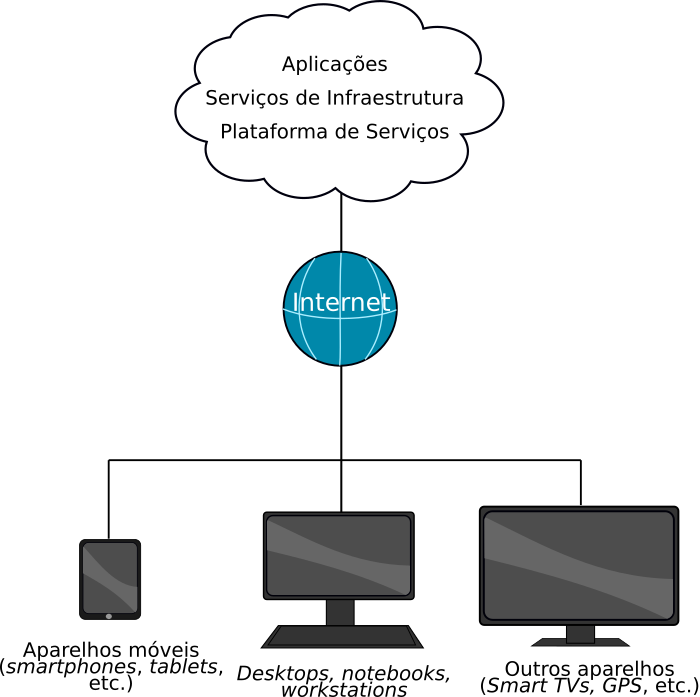
\includegraphics[scale=0.5]{compnuvem}
	\centering
	\label{fig:compnuvem}
\end{figure}

Em 2011, o \emph{Information Technology Laboratory} (ITL), que faz parte \emph{National Institute of Standards and Technology} (NIST), uma agência governamental que promove a utilização de padrões em ambientes de tecnologia da informação, lançou um documento que define a computação em nuvem como ``um modelo que permite acesso ubíquo, conveniente e sob demanda para uma gama de recursos computacionais compartilhados que podem ser provisionados e liberados com o mínimo de esforço ou interação do provedor de serviço.'' \cite[p. 2]{mell2011nist} (Tradução adaptada pelo autor).

O documento também prevê cinco características essenciais, três modelos de serviço e quatro modelos de implementação que definem o ambiente de computação em nuvem, que serão descritas nas subseções a seguir, de acordo com as definições propostas no documento.

\subsection{Características essenciais}

O documento define as seguintes características essenciais para ambientes de computação em nuvem:
\begin{itemize}
	\item \textbf{Atendimento sob demanda:} O consumidor pode requisitar as operações do serviço em tempo real, como armazenamento de dados por exemplo, sem necessidade de interação humana com o provedor de serviços.
	\item \textbf{Amplo acesso à rede:} Os serviços são disponibilizados por meio do acesso à internet, utilizando mecanismos padronizados que permitam o acesso utilizando diferentes plataformas, como celulares, \emph{notebooks}, \emph{tablets}, \emph{desktops} etc.
	\item \textbf{\emph{Pool} de recursos:} Os recursos computacionais do provedor de serviços deve ser capaz de servir múltiplos consumidores ao mesmo tempo, com diferentes recursos físicos e virtuais sendo destinados dinamicamente de acordo com a demanda do consumidor.
	\item \textbf{Rápida elasticidade:} Os recursos computacionais podem ser fornecidos e liberados de forma elástica, em alguns casos de forma automática, escalando de forma adequada conforme a demanda. Para o consumidor, tais recursos podem parecer ilimitados, ou então podem ser adquiridos em qualquer quantidade a qualquer tempo.
	\item \textbf{Serviços mensuráveis:} Sistemas de nuvem controlam e otimizam automaticamente o uso de recursos utilizando recursos mensuráveis (que geralmente são alcançados utilizando um serviço de ``pagar por uso''). O uso de recursos pode ser monitorado, controlado, e reportado, promovendo transparência tanto para o consumidor quanto para o provedor de serviços.
\end{itemize}

\subsection{Modelos de serviço}

Os modelos de serviço definidos no documento estão descritos a seguir, com tradução e adaptação pelo autor:

\begin{itemize}
	\item \textbf{\emph{Software as a Service (SaaS)}:} O recurso computacional é disponibilizado para o consumidor como uma aplicação executada em infraestrutura na nuvem. Essa aplicação pode ser acessada de diversos dispositivos, podendo-se utilizar um navegador de internet, ou até mesmo uma aplicação própria. O consumidor, neste caso, não tem nenhum controle sobre os servidores, sistemas operacionais, armazenamento ou aplicações que fazem parte da infraestrutura da rede, limitando-se apenas àquilo que lhe foi designado como serviço disponível.
	\item \textbf{\emph{Platform as a Service (PaaS)}:} O recurso disponibilizado ao consumidor é para a implementação de um sistema de computação em nuvem, podendo assim criar sua prórpia aplicação ou serviço utilizando a infraestrutura existente. Neste caso, o consumidor também não possui controle sobre tal infraestrutura, mas pode implementar aplicações e configurações no ambiente hospedeiro.
	\item \textbf{\emph{Infrastructure as a Service (IaaS)}:} O recurso computacional disponibilizado é prover processamento, armazenamento, rede e outros recursos fundamentais onde o consumidor pode implementar e executar sistemas operacionais e aplicações a seu gosto, quando disponíveis. O consumidor também não controla a infraestrutura, mas já tem controle sobre os sistemas operacionais, armazenamento e aplicações implementadas.
\end{itemize}


\subsection{Modelos de implementação}

\begin{itemize}
	\item \textbf{Nuvem privada:} A infraestrutura em nuvem provisionada é de uso exclusivo de uma organização, compondo-se de múltiplos consumidores.
	\item \textbf{Nuvem comunitária:} A infraestrutura em nuvem provisionada é de uso exclusivo de uma comunidade específica de consumidores de organizações com interesses em comum.
	\item \textbf{Nuvem pública:} A infraestrutura em nuvem provisionada é aberta para o público em geral.
	\item \textbf{Nuvem híbrida:} A infraestrutura em nuvem disponibilizada é uma composição de duas ou mais infraestruturas de nuvem descritas anteriormente, que continuam operando de forma independente, mas que se interconectam por uma tecnologia padronizada que permite a portabilidade de aplicações e dados.
\end{itemize}

\subsection{Aplicações na indústria}

Existem inúmeras aplicações de computação em nuvem na indústria, que variam de acordo com a natureza da indústria e sua carga de trabalho \cite[p. 10]{khan2018cloud}.

Nesta seção, serão apresentados alguns serviços mais conhecidos e relevantes de computação em nuvem, mas não necessariamente são os únicos disponíveis.

\subsubsection{\emph{Amazon Web Services (AWS)}}

Amazon Web Services (AWS) \cite{aws} é um conjunto de serviços de nuvem, que fornecem computação baseada em nuvem, armazenamento e outras aplicações que atendem tanto o aspecto corporativo quanto a usuários individuais. Nesse ambiente, usuários podem implementar aplicações e serviços sob demanda, pagando de acordo com o uso. \cite[p. 13]{zhang2010cloud}

Neste contexto, a Amazon disponibiliza também o serviço conhecido como \emph{\textbf{Amazon Elastic Compute Cloud}}, também chamado de \textbf{Amazon EC2}. Segundo o próprio serviço: ``O Amazon Elastic Compute Cloud (Amazon EC2) é um web service que disponibiliza capacidade computacional segura e redimensionável na nuvem. Ele foi projetado para facilitar a computação em nuvem na escala da web para os desenvolvedores.'' \cite{amazonec2}. Tal plataforma permite que o usuário administre servidores e \emph{data centers} utilizando APIs ou ferramentas e utilitários disponíveis. As instâncias da EC2 são máquinas virtuais sendo executadas dentro da engine de virtualização Xen \cite{xenengine} \cite{zhang2010cloud}.

A estrutura da AWS também comporta serviços como o Amazon Virtural Private Cloud (VPC), que se comporta como uma rede privada virtual (VPN), utilizando os recursos da AWS para permitir uma segurança adicional para o usuário final, com serviços de firewall, detecção de intrusão, entre outros serviços.

\subsubsection{Microsoft Azure}

A plataforma Microsoft Azure, antigamente chamada de Microsoft Windows Azure, consiste em uma plataforma da própria Microsoft para executar aplicações e armazenar dados na nuvem \cite{chappell2009introducing}. Os produtos permitem o armazenamento de dados em nuvem, execução de aplicações, gerenciamento de contâineres, APIs de detecção facial, ferramentas de testes para desenvolvedores, entre outras aplicações \cite{microsoftazure}.

Os serviços do Microsoft Azure têm sido utilizados em diversas áreas distintas, como geoprocessamento \cite{gong2010geoprocessing}, predição de estruturas de proteínas em 3D \cite{mrozek2015scaling}, utilização de aprendizado de máquina em pesquisa de radiologia \cite{kohli2017implementing}, entre outras tantas aplicações disponíveis na literatura.

\section{Tolerância a falhas}

O uso de sistemas computacionais é ubíquo no mundo moderno, extendendo-se a aplicações em sistemas de defesa, sistemas aéreo, controle de tráfego aéreo, sistemas bancários, jogos virtuais, dentre tantos outros. A variedade de aplicações e a importância crescente desse setor trouxe à tona a confiabilidade de sistemas computacionais para as mais diversas aplicações. \cite{andersonfault}

Um exemplo de preocupação com o funcionamento adequado desses sistemas ocorreu no fim da década de 1990, quando percebeu-se o modo ineficiente de armazenamento e formatação de datas de calendários em sistemas computacionais da época, e que colocaria em risco a correta execução de milhares de serviços dependentes desses sistemas, podendo também ocasionar uma pane geral de alguns sistemas de alto risco. Tal episódio é conhecido na literatura como ``Problema do Ano 2000'', muitas vezes estilizado como ``Y2K \emph{problem}'', ou popularmente chamado de ``\emph{Bug} do Milênio'' . A preocupação com uma pane em massa de praticamente todos os sistemas computacionais levou a criação de uma série de medidas para garantir a correção desse problema nos sistemas existentes e prevenir a ocorrência de problemas similares em futuros sistemas desenvolvidos \cite{petersen1998y2k}.

Este clássico exemplo de prevenção de falhas mostra uma fraqueza de alguns sistemas computacionais em lidar com falhas previstas anteriormente. Caso tais correções e recomendações não fossem consideradas, especula-se que as consequências poderiam ser catastróficas para os mais diversos setores que dependiam desses sistemas computacionais \cite{smith1997year}. Assim sendo, deve-se levar em consideração que existem problemas aos quais sistemas computacionais estão sujeitos, mas que podem ser tratados adequadamente em tempo de execução, evitando ao máximo comprometer o funcionamento desse sistema.

\subsection{Conceitos básicos}

Assim como os sistemas mencionados anteriormente estavam sujeitos a falhas causadas por uma falta de planejamento dos desenvolvedores, sistemas computacionais estão sujeitos a inúmeros tipos de falhas, que podem fugir completamente ao controle tanto de administradores do sistema quanto aos desenvolvedores ou fabricantes de tal produto.

Desenhar um sistema computacional que permita uma recuperação em meio a uma falha ou então que permita ao administrador corrigir tal falha sem comprometer o funcionamento de todo um serviço é uma das grandes prioridades para qualquer pessoa que almeja projetar tais sistemas \cite{bala2012fault}. É neste contexto que surge o conceito de tolerância a falhas.

Tal conceito em computação é bastante antigo e se aplica tanto no âmbito do fabricante de \emph{hardware} quanto na área de desenvolvimento de \emph{software} \cite{randell1975system}. Para ambos, é importante garantir a confiabilidade do sistema para qualquer um que venha a utilizá-lo posteriormente.


\subsection{Modelos de falhas}



\subsection{Técnicas de tolerância a falhas}



\subsubsection{Técnicas reativas}



\subsubsection{Técnicas proativas}




\subsection{Aplicações}


\subsection{}

% ---

% ---
\section{Sistemas de recomendação}\label{sec_recom}


\subsection{Conceitos básicos}

Sistemas de recomendação são um conjunto de técnicas e ferramentas que fornecem sugestões de itens que podem ser úteis para o usuário final \cite{resnick1997recommender} \cite{good1999combining} \cite{burke2007hybrid}. Amplamente utilizados na indústria de computação, os sistemas de recomendação tem ganhado cada vez mais notoriedade com o crescente uso de \emph{Data mining} por parte de gigantes da computação, como a Google, Facebook e Amazon, por exemplo.

INSERIR DIAGRAMA AQUI..



\subsection{Aplicações}

O uso de tecnologias de recomendação é bastante presente em plataformas de computação em nuvem, e mostram-se bastante eficazes na arte de influenciar o usuário final a tomar uma decisão baseada naquilo que lhe é sugerido. Um bom exemplo do uso de sistemas de recomendação nesse âmbito é o algoritmo de recomendação de vídeos utilizado pelo YouTube. Um estudo realizado em 2010 \cite{zhou2010impact}, mostra uma correlação entre o sistema de recomendação de vídeos do YouTube e as visualizações de cada vídeo afetado.

Sistemas como esse também são amplamente utilizados na área do comércio virtual, mais conhecido como \emph{e-commerce}, fazendo a sugestão de produtos e anúncios para usuários que demonstram interesses em determinadas categorias pela internet. No decorrer desta sessão, será discutido de forma mais aprofundada sobre essa área de utilização, e serão apresentados modelos de negócios específicos que utilizam sistemas de recomendação e detalhes desses sistemas.

O uso de um sistema de recomendação varia de acordo com o modelo de negócio utilizados e sua plataforma necessária para funcionamento.


\subsubsection{\emph{E-commerce}}

Uma das maiores áreas que utilizam sistemas de recomendação é o âmbito do \emph{e-commerce}, conhecido também como comércio virtual \cite{schafer1999recommender}. Neste, destacam-se grandes nomes do varejo e vendas em geral como Walmart, Carrefour, Saraiva, Casas Bahia, Pontofrio etc. e outras empresas focadas exclusivamente no comércio virtual como Amazon, Mercado Livre, KaBuM, dentre outras tantas que surgiram nos últimos anos. \cite{schafer2001commerce}

A utilização de sistemas de recomendação inteligentes provou ser um importante aliado para a obtenção de lucro para empresas desse tipo, já que as recomendações oferecidas são adaptadas de cliente para cliente, adaptando-se de acordo com os gostos explicitados pelo cliente.

\subsection{Técnicas}

\section{Considerações finais}

\chapter{Projeto}\label{cap_projeto}

Capítulo de descrição do projeto de implementação do sistema de recomendação trabalhado.
% ---

% ----------------------------------------------------------
% Finaliza a parte no bookmark do PDF
% para que se inicie o bookmark na raiz
% e adiciona espaço de parte no Sumário
% ----------------------------------------------------------
\phantompart

% ---
% Conclusão
% ---
\chapter{Conclusão}
% ---


% ----------------------------------------------------------
% ELEMENTOS PÓS-TEXTUAIS
% ----------------------------------------------------------
\postextual
% ----------------------------------------------------------

% ----------------------------------------------------------
% Referências bibliográficas
% ----------------------------------------------------------
\bibliography{referencias}

% ----------------------------------------------------------
% Glossário
% ----------------------------------------------------------
%
% Consulte o manual da classe abntex2 para orientações sobre o glossário.
%
%\glossary

% ----------------------------------------------------------
% Apêndices
% ----------------------------------------------------------

% ---
% Inicia os apêndices
% ---
\begin{apendicesenv}

% Imprime uma página indicando o início dos apêndices
\partapendices

% ----------------------------------------------------------
\chapter{Quisque libero justo}
% ----------------------------------------------------------

\lipsum[50]

\end{apendicesenv}
% ---


% ----------------------------------------------------------
% Anexos
% ----------------------------------------------------------

% ---
% Inicia os anexos
% ---
\begin{anexosenv}

% Imprime uma página indicando o início dos anexos
\partanexos

% ---
\chapter{Morbi ultrices rutrum lorem.}
% ---
\lipsum[30]

\end{anexosenv}

%---------------------------------------------------------------------
% INDICE REMISSIVO
%---------------------------------------------------------------------
\phantompart
\printindex
%---------------------------------------------------------------------

\end{document}
